% Drawing 146/06-1 -- folder 146, batch 06, archive page 112 (PDF page 113).
% Transcription: dans la marge gauche, une sphère avec son équateur et un triangle inscrit en pointillé ; au-dessous, un cercle portant les points $\infty$ (en haut), $0$ et $1$, un petit cercle autour de $0$ et des segments en pointillé.
% Kind: sphere with inscribed triangle; circle 0, 1, infinity. Method 2 (schematic redraw from the facsimile). Status: partial.
% Notes: Sphere with its equator (back half dashed) and a dashed triangle inscribed; the circle with infinity at the top, 0 at the lower left with a small circle round it, dashed segments and two thick arcs. Only infinity is legible on the crop; 0 is placed at the point carrying the small circle, as the transcription implies; the point labelled 1 (bottom or right?) cannot be told and 1 is not placed.
% Coordinates: 1 unit = 1 mm = 1/100 of the crop width (bbox in page fractions: [0.12, 0.64, 0.32, 0.87]).
% Redrawn by Claude (claude-opus-5-5), issue #73 pilot, 2026-11-07; not checked by a human; not compiled (no TeX in the session).
% Rights: reproduces part of the work -- behind RENDER_TRANSCRIPTS, never published by itself.
\documentclass[tikz,border=3pt]{standalone}
\usepackage{amsmath,amssymb}
\usetikzlibrary{patterns,arrows.meta}
\tikzset{pencil/.style={black!45}, struck/.style={black!35}, mark/.style={circle,draw,inner sep=1.3pt}, pt/.style={circle,fill,inner sep=0.9pt}, opt/.style={circle,draw,fill=white,inner sep=1.1pt}}
\begin{document}
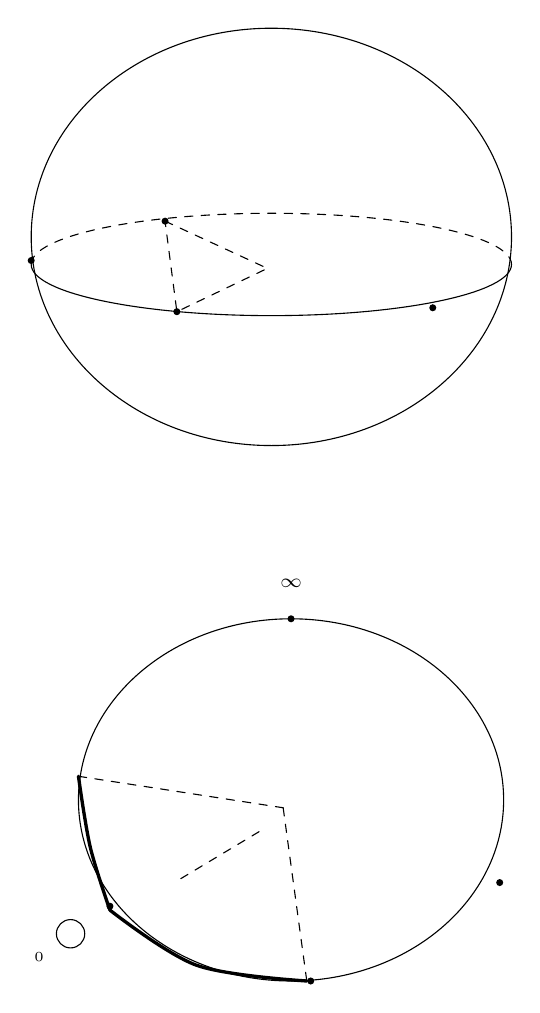
\begin{tikzpicture}[x=1mm,y=1mm,line cap=round,line join=round,font=\scriptsize]
\draw (49.5,-44.5) ellipse[x radius=30.5, y radius=26.5];
\draw (19,-48) arc[start angle=180, end angle=360, x radius=30.5, y radius=6.5];
\draw[dashed] (80,-48) arc[start angle=0, end angle=180, x radius=30.5, y radius=6.5];
\draw[dashed] (36,-42.5) -- (49,-48.5) -- (37.5,-54) -- cycle;
\node[pt] at (36,-42.5) {};
\node[pt] at (37.5,-54) {};
\node[pt] at (70,-53.5) {};
\node[pt] at (19,-47.5) {};
\draw (52,-116) ellipse[x radius=27, y radius=23];
\node[pt] at (52,-93) {};
\node[inner sep=1pt] at (52,-88.5) {\scriptsize $\infty$};
\node[pt] at (29,-129.5) {};
\draw (24,-133) circle[radius=1.8];
\node[inner sep=1pt] at (20,-136) {\tiny $0$};
\node[pt] at (54.5,-139) {};
\node[pt] at (78.5,-126.5) {};
\draw[dashed] (25,-113) -- (51,-117);
\draw[dashed] (51,-117) -- (54,-139);
\draw[dashed] (38,-126) -- (48,-120);
\draw[very thick] plot[smooth, tension=0.55] coordinates {(25,-113) (26.5,-122) (29,-130)};
\draw[very thick] plot[smooth, tension=0.55] coordinates {(29,-130) (40,-137) (54,-139)};
\end{tikzpicture}
\end{document}
